\section{Main Results}
\label{sec:main_results}

We evaluate 14 state-of-the-art LLMs on GPSBench across two tracks: the Applied Track (8 tasks testing real-world geographic reasoning) and the Pure GPS Track (9 tasks testing coordinate manipulation).

%% =============================================================================
\subsection{RQ1: How Well Do LLMs Perform on GPS Reasoning Tasks?}
\label{sec:rq1_overall_performance}

\begin{figure}[htbp]
\centering
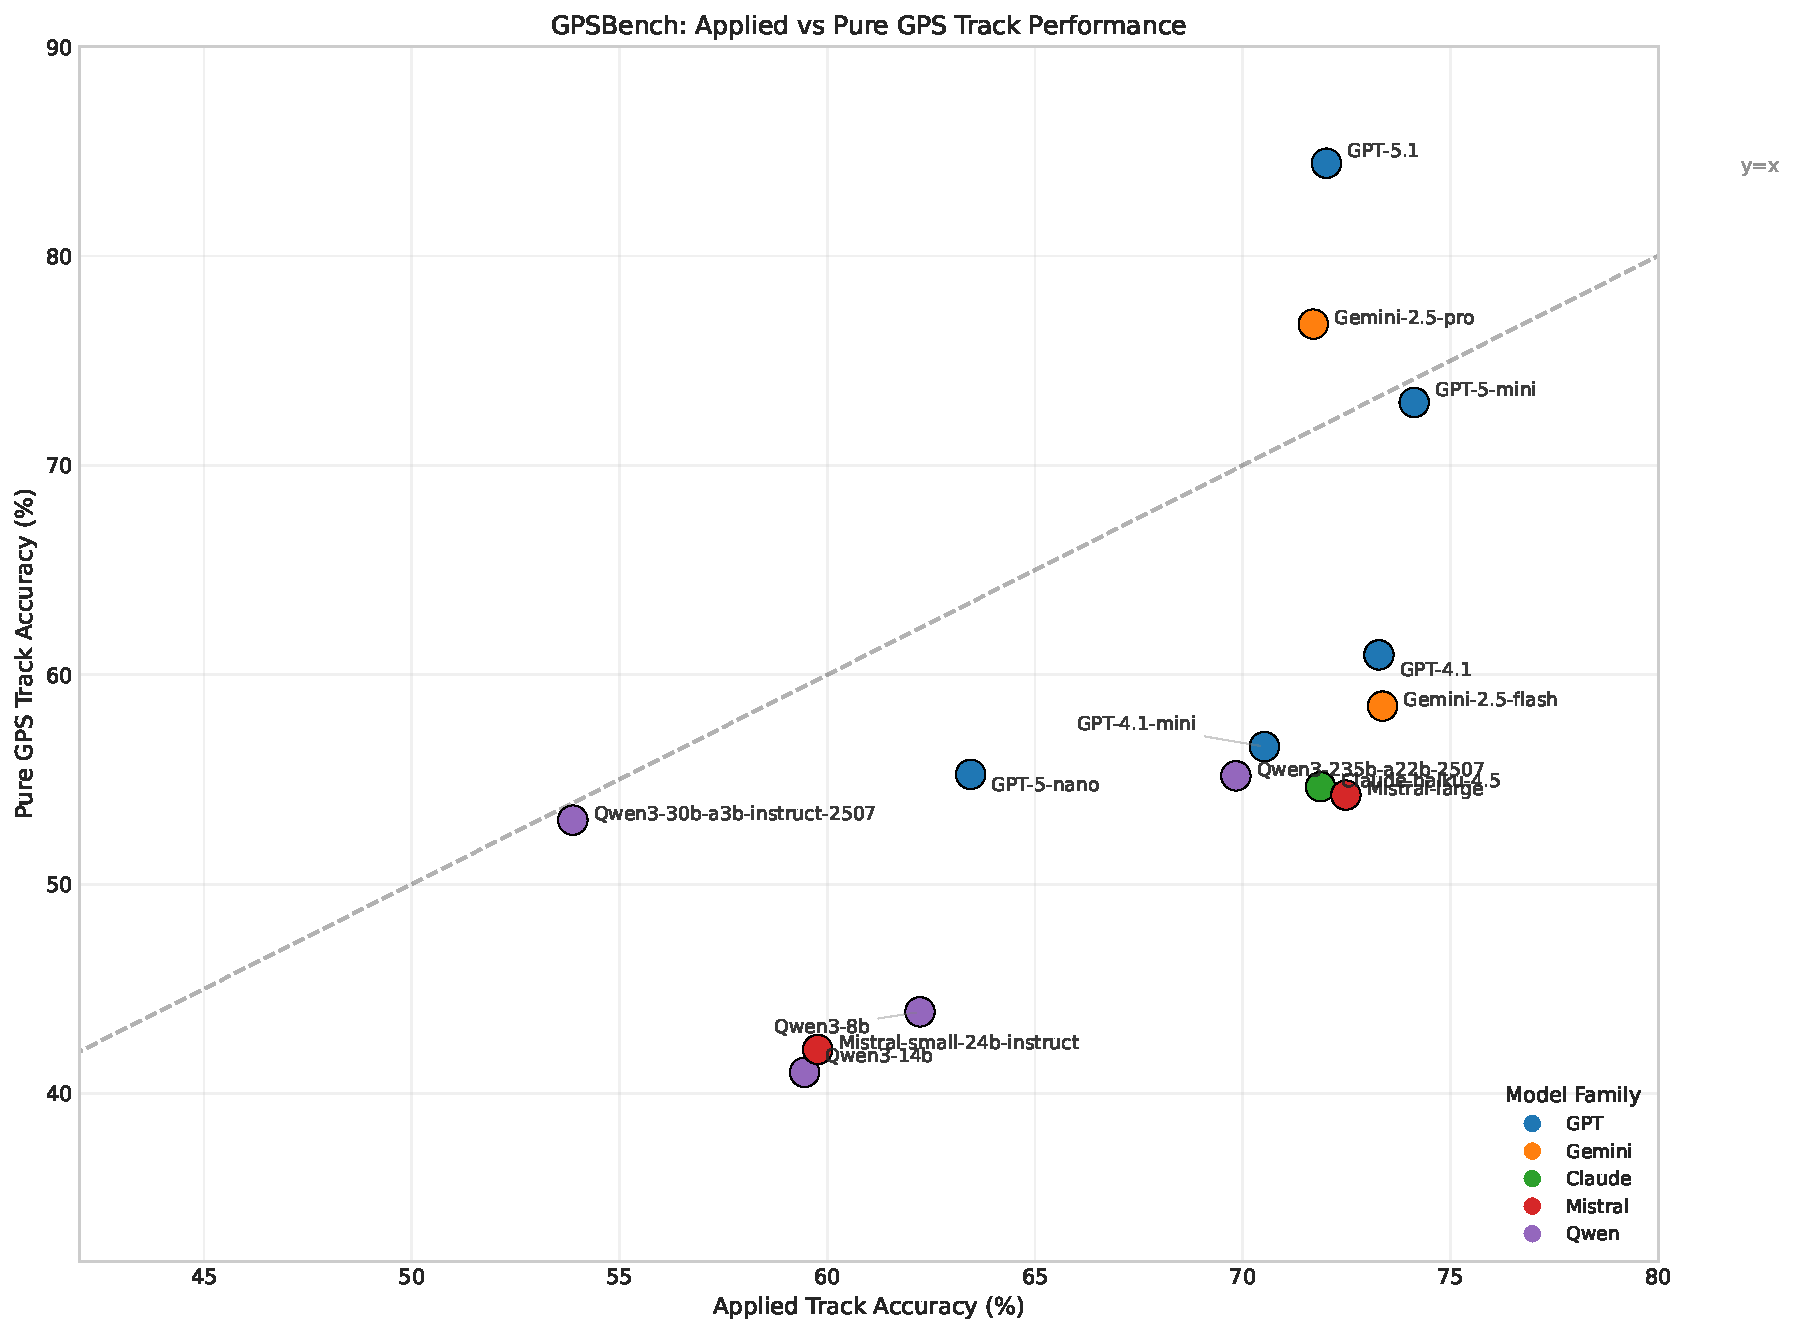
\includegraphics[width=\columnwidth]{figures/main_results_scatter.pdf}
\caption{Applied vs Pure GPS Track performance. Most models cluster below the diagonal (favoring Applied), while GPT-5.1 and Gemini-2.5-Pro uniquely excel at Pure GPS computation.}
\label{fig:scatter}
\end{figure}

\paragraph{Overall Performance.}
As shown in Figure~\ref{fig:scatter}, GPT-5-mini achieves the highest Applied Track accuracy (74.1\%), followed by Gemini-2.5-Flash (73.4\%) and GPT-4.1 (73.3\%). On the Pure GPS Track, GPT-5.1 leads with 84.4\%, followed by Gemini-2.5-Pro (76.7\%). The overall mean across 14 models is 67.7\% for Applied and 57.8\% for Pure GPS, with a +9.9\% gap favoring Applied tasks (see Appendix~\ref{app:overall_results} for full results).

\paragraph{Model Family Patterns.}
Model families exhibit distinct capability profiles. GPT and Gemini families show balanced performance with small Applied-Pure gaps (4--5\%), while Mistral, Claude, and Qwen families show larger gaps (13--18\%), excelling at world-knowledge tasks but struggling with coordinate computation. Notably, only two models exceed the diagonal in Figure~\ref{fig:scatter}: GPT-5.1 (Pure GPS $>$ Applied by 12.4\%) and Gemini-2.5-Pro (by 5.0\%), suggesting these flagship models have strong mathematical reasoning capabilities.

\begin{figure}[htbp]
\centering
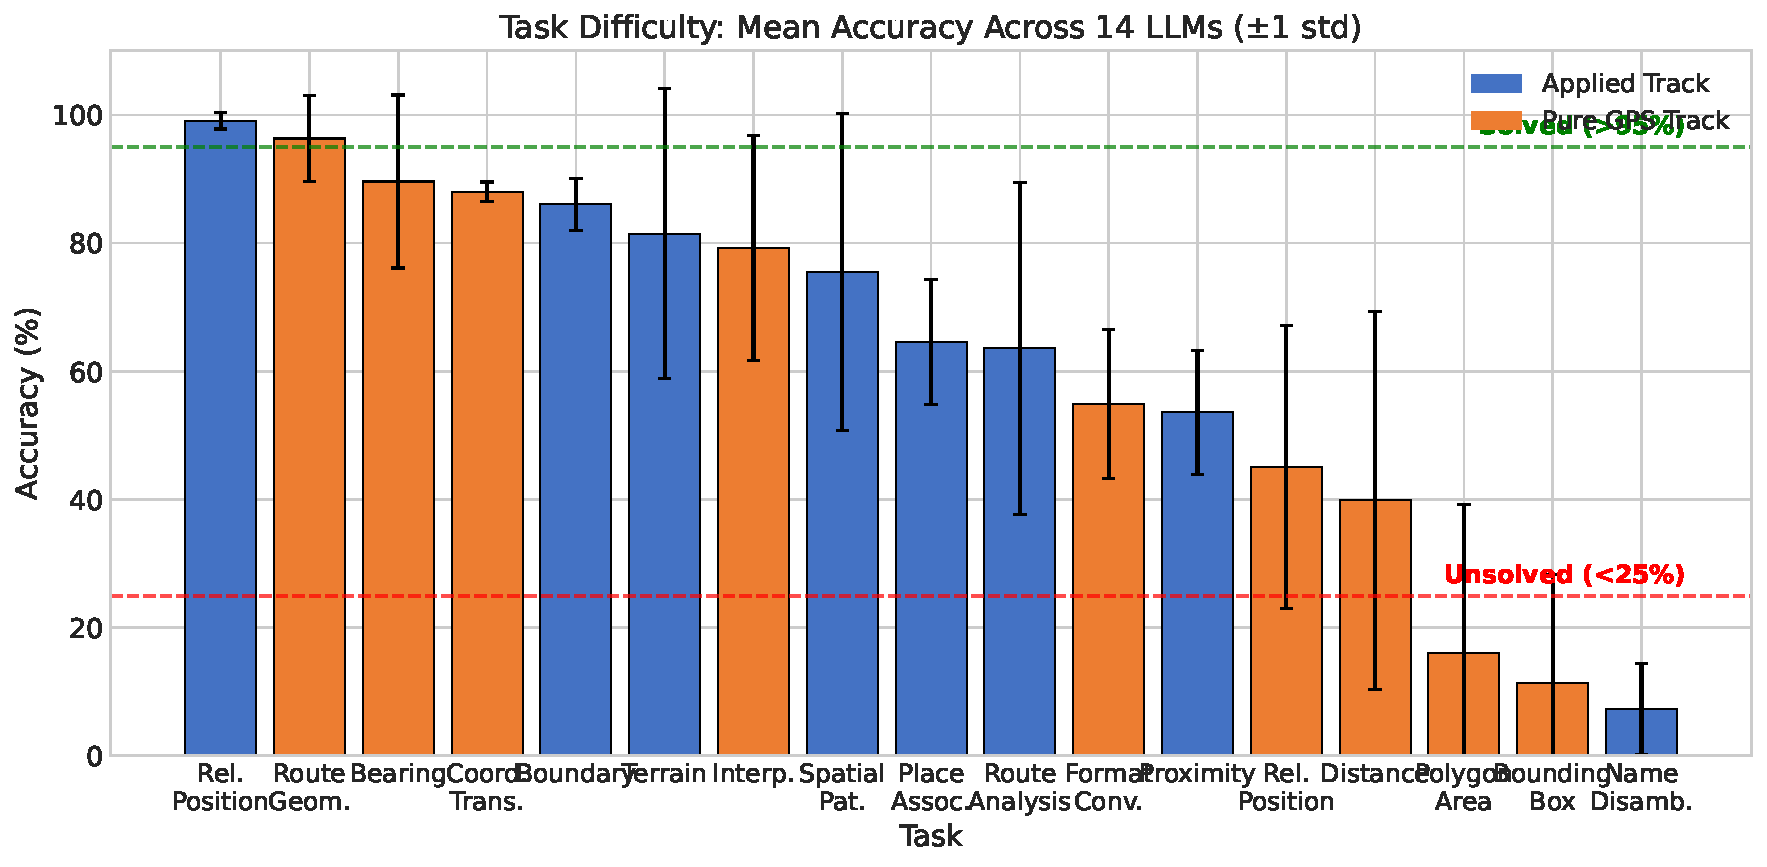
\includegraphics[width=\columnwidth]{figures/task_difficulty_average.pdf}
\caption{Mean accuracy across 14 LLMs per task, sorted by difficulty. Error bars show $\pm$1 standard deviation. Tasks cluster into solved ($>$95\%), brittle (25--95\%), and unsolved ($<$25\%) tiers.}
\label{fig:task_difficulty}
\end{figure}

\paragraph{Task Difficulty.}
Figure~\ref{fig:task_difficulty} reveals that task difficulty correlates with knowledge type rather than computational complexity. Tasks cluster into three tiers. \textit{Solved tasks} ($>$95\%) include Name Disambiguation and Bounding Box, which can be addressed through pattern matching or simple heuristics. \textit{Brittle tasks} (25--95\%) such as Distance Calculation, Coordinate Transformation, and Spatial Patterns show high variance across models, indicating these capabilities are unevenly distributed; some models excel while others fail entirely. \textit{Unsolved tasks} ($<$25\%) include Place Association, Polygon Area, and Coordinate Interpolation, representing fundamental capability gaps. Place Association requires dense coordinate-to-city mappings absent from training data, while Polygon Area and Interpolation demand multi-step spherical geometry reasoning. Notably, Polygon Area fails despite being purely mathematical, revealing that models have not learned geodetic formulas like L'Huilier's theorem. Qualitative error analysis reveals three failure modes: (1) knowledge gaps, where models substitute nearby prominent cities for exact locations (e.g., coordinates for Emure-Ekiti, Nigeria yield ``Akure, Ondo State''---the state capital 50km away); (2) computational complexity, where multi-step geodetic calculations accumulate numerical errors (e.g., a polygon area of 371,518 km\textsuperscript{2} is estimated as 2,200,000 km\textsuperscript{2}); and (3) geographic bias, where models default to well-known locations when city names are ambiguous (e.g., assuming ``Rye'' refers to the English town rather than Rye, Australia, causing the model to misidentify the geographic outlier). See Appendix~\ref{app:error_analysis} for detailed patterns.

\paragraph{Flagship Models Excel at Coordinate Computation.}
GPT-5.1 achieves 84.4\% Pure GPS accuracy, surpassing GPT-5-mini (73.0\%) by 11.4\%. It dominates 5 of 9 Pure GPS tasks: Distance (99.9\%), Bearing (99.9\%), Route Geometry (96.3\%), Coordinate Transformation (90.8\%), and Interpolation (71.4\%). In contrast, Gemini-2.5-Pro leads on Applied tasks requiring world knowledge: Spatial Patterns (95.4\%) and Place Association (23.0\%, the highest among all models). This bifurcation suggests GPS reasoning comprises two distinct capabilities: (1) geometric computation, where flagship models with strong mathematical training excel, and (2) geographic knowledge integration, where models with broad world knowledge have advantages.

\begin{figure}[htbp]
\centering
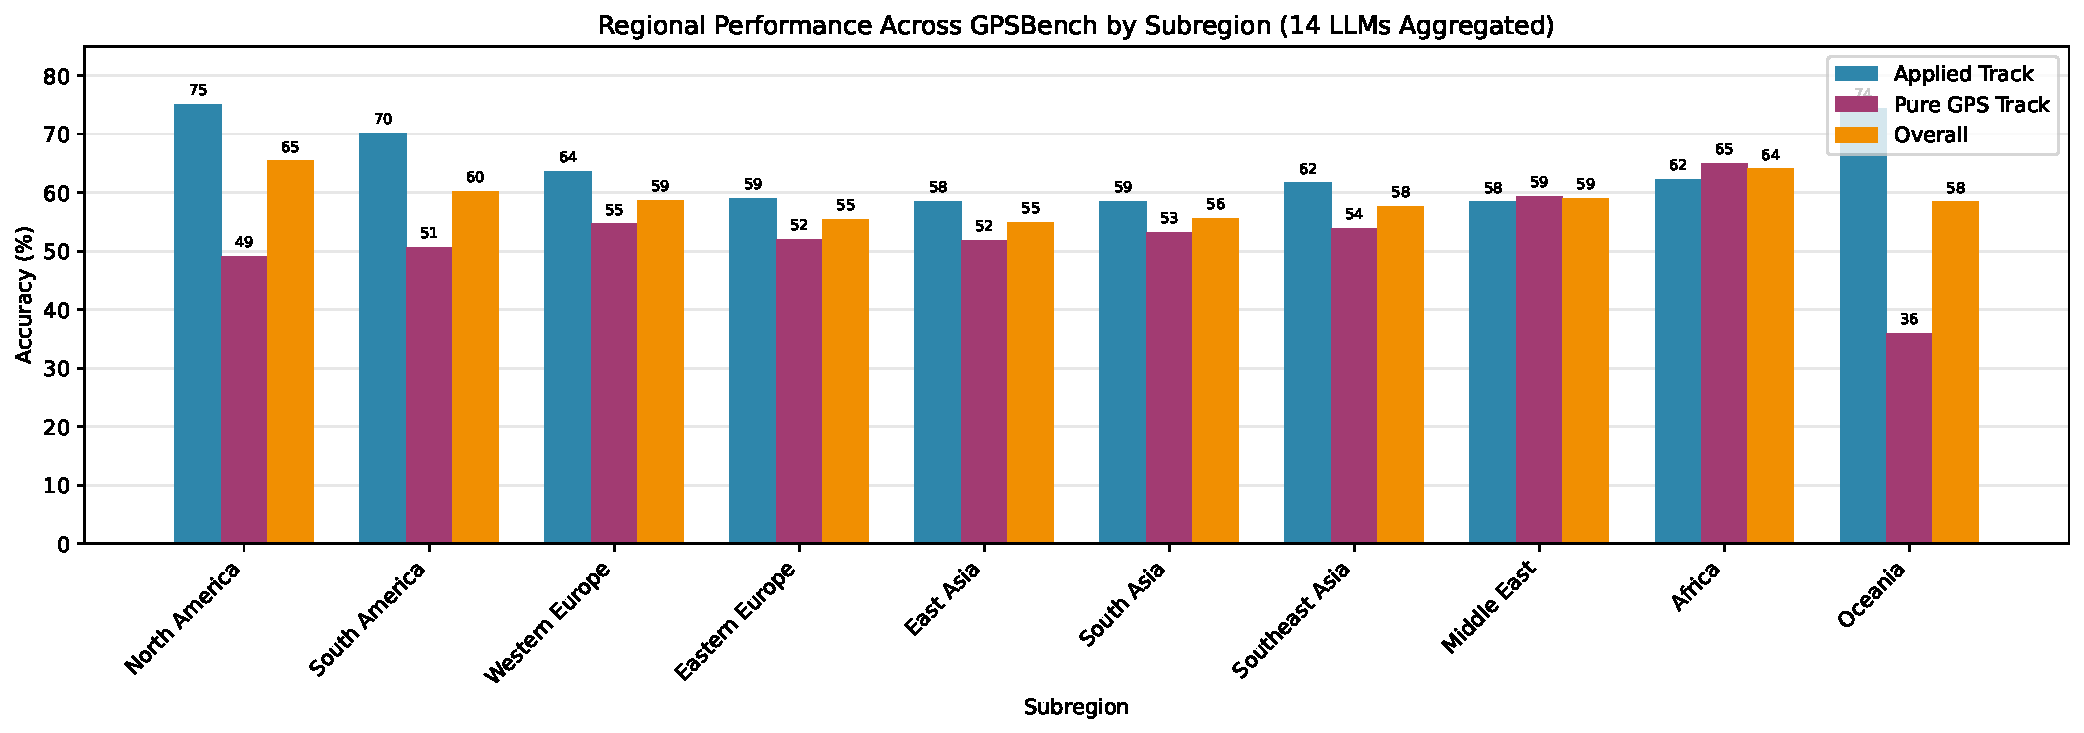
\includegraphics[width=\columnwidth]{figures/regional_performance_subregion.pdf}
\caption{Regional performance by subregion across all GPSBench tasks (14 LLMs aggregated). Applied Track shows the largest gaps: North America (75.1\%) vs.\ East Asia (58.5\%), a 16.6\% difference. Pure GPS Track is more uniform across most subregions.}
\label{fig:regional_subregion}
\end{figure}

\paragraph{Geographic Bias is Task-Specific.}
We analyze regional performance across all 17 tasks by subregion (Figure~\ref{fig:regional_subregion}). Overall accuracy varies by 10.5\% across subregions (North America 65.4\% vs.\ East Asia 55.0\%), but this masks substantial track-specific patterns. The Applied Track shows larger variation (16.6\% gap): North America (75.1\%) and Oceania (74.5\%) outperform East Asia (58.5\%) and Middle East (58.4\%). For Place Association specifically, the disparity is even starker: North America (14.7\%) and Western Europe (11.0\%) outperform South Asia (2.6\%) and East Asia (3.8\%) by 4--6$\times$. In contrast, Pure GPS computation tasks show minimal regional bias across most subregions: Distance Calculation (74.6--83.3\%), Bounding Box (95.2--98.5\%), and Format Conversion (97.4--100\%) vary by $<$9\% across all subregions. This confirms that geographic bias stems from sparse coordinate-to-place mappings in training data, not computational limitations. Location-aware applications using world knowledge will perform substantially worse in underrepresented regions, while pure geometric computation remains reliable globally (see Appendix~\ref{app:regional_performance} for per-task breakdown).

%% =============================================================================
\subsection{RQ2: How Does Geographic Granularity Affect Performance?}
\label{sec:rq2_granularity_robustness}

We investigate how performance varies across geographic granularity levels and whether coordinate noise affects model accuracy, using Place Association as a probe task.

\begin{figure}[htbp]
\centering
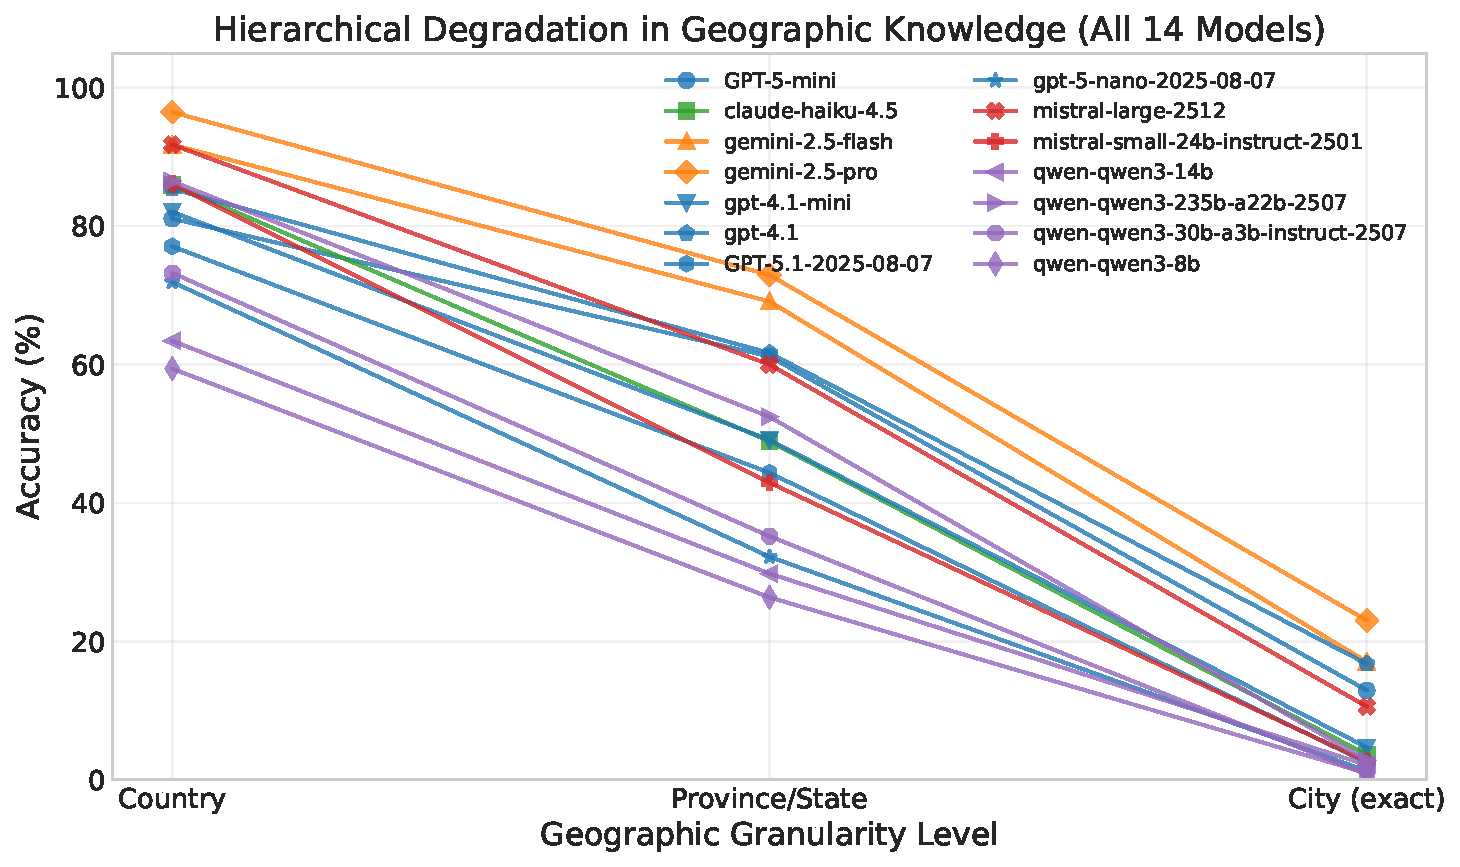
\includegraphics[width=\columnwidth]{figures/place_association_granularity_line.pdf}
\caption{Hierarchical degradation in geographic knowledge. Models perform well at country-level but accuracy drops sharply for finer granularities, with city-level accuracy below 25\% for all models.}
\label{fig:place_assoc_granularity}
\end{figure}

\paragraph{Hierarchical Degradation.}
As shown in Figure~\ref{fig:place_assoc_granularity}, models exhibit clear hierarchical degradation. Country-level identification ranges from 59--97\%, province/state drops to 26--73\%, and exact city identification collapses to 1--23\%. This reveals that LLMs encode geographic knowledge at coarse spatial resolutions but lack the dense mappings needed for city-level localization (see Appendix~\ref{app:granularity_full} for full results).

\paragraph{Robustness to Coordinate Noise.}
We apply Gaussian noise ($\sigma \in \{0, 10, 50, 100, 500, 1000\}$m) to coordinates, representing conditions from precise GPS ($\pm$10m) to coarse IP geolocation ($\pm$1km). Each noise level contains $\sim$567 samples. This tests both coordinate precision sensitivity and memorization: if models memorized specific coordinate$\rightarrow$place mappings, noise would break these associations and degrade performance. Crucially, we analyze this at all granularity levels (Figure~\ref{fig:noise_granularity}). Country-level accuracy remains stable at 79--82\% across all noise levels ($\Delta$: $\pm$1.6\%), province-level at 46--52\% ($\Delta$: $\pm$5.8\%), and city-level at 6--9\% ($\Delta$: $\pm$2\%). The absence of degradation at any granularity level, even for high-accuracy country identification, suggests models genuinely understand the GPS coordinate system rather than relying on memorized coordinate strings.

\paragraph{Error Analysis.}
Across all 14 models, we analyze the 92.7\% of predictions that fail at city-level identification. Of these errors, 80.4\% still identify the correct country, while only 19.6\% miss the country entirely. Per-model breakdown shows consistent patterns: even low-performing models like Qwen3-8B (1.0\% city accuracy) achieve 59.4\% country identification, while top performers like Gemini-2.5-Pro reach 96.8\% country accuracy (23.0\% city + 73.8\% country-only). This indicates models have reasonable coarse geographic knowledge but lack the dense coordinate$\rightarrow$city mappings needed for fine-grained localization. Combined with noise robustness, this confirms that the bottleneck is sparse city-level knowledge in model training data, not coordinate understanding or memorization.

\paragraph{GeoNames Memorization Probe.}
To directly test whether models have memorized exact coordinates from geographic databases like GeoNames, we designed a Missing Data task requiring models to infer coordinates given city names (e.g., ``What is the latitude of Springfield, Illinois?''). If models memorized the GeoNames dataset, they should achieve high accuracy with $\pm$0.1° tolerance. Results show uniformly low performance across all models (mean: 8.3\%), with even top performers like Gemini-2.5-Pro achieving only 12.4\%. This confirms that LLMs have not memorized coordinate databases: they possess coarse geographic knowledge (country/continent level) but lack the dense coordinate-place mappings that would result from database memorization.

\begin{figure}[htbp]
\centering
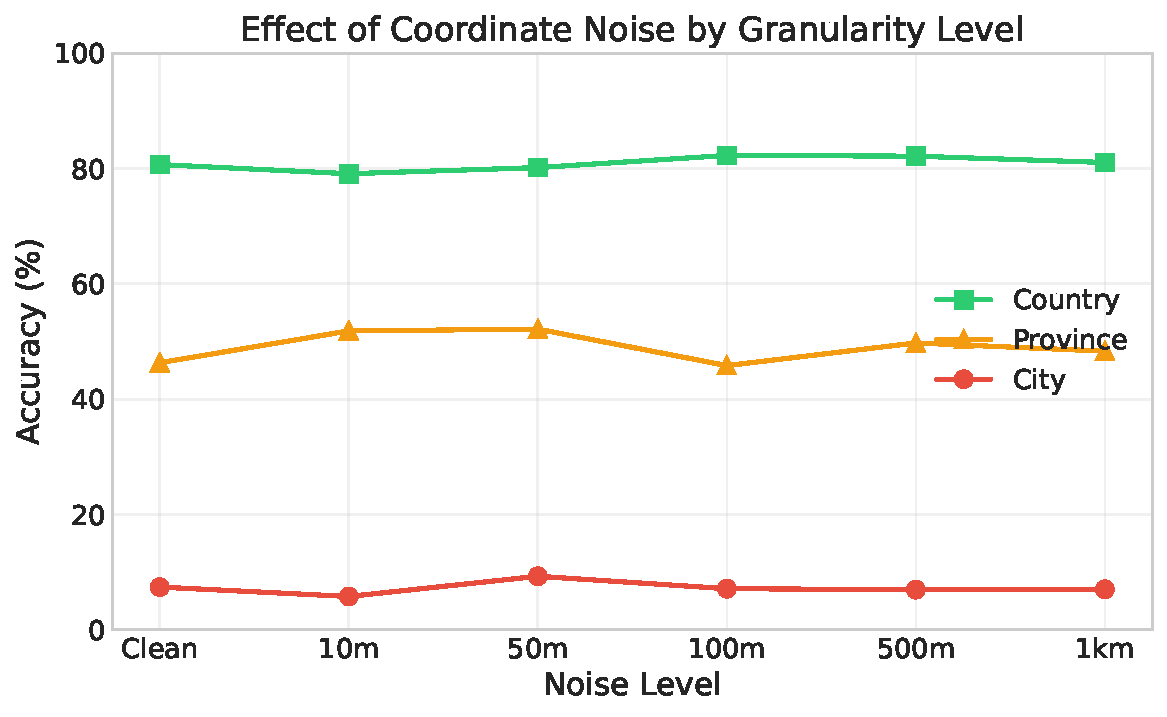
\includegraphics[width=\columnwidth]{figures/place_association_noise_by_granularity.pdf}
\caption{Effect of coordinate noise across granularity levels. All levels show flat performance regardless of noise magnitude (10m to 1km), suggesting models rely on generalized geographic knowledge rather than memorized coordinate$\rightarrow$place mappings.}
\label{fig:noise_granularity}
\end{figure}

%% =============================================================================
\subsection{RQ3: Does GPS Augmentation Improve Downstream Tasks?}
\label{sec:rq3_downstream_gps_augmentation}

Given that LLMs can process GPS coordinates for many tasks (RQ1), we investigate whether augmenting existing geographic reasoning benchmarks with explicit coordinates improves performance.

\paragraph{Datasets.}
We evaluate on two benchmarks that test different aspects of geographic reasoning:
\begin{itemize}[leftmargin=*, itemsep=2pt]
    \item \textbf{MapEval}~\cite{mapeval}: A benchmark of 200 map-based questions requiring spatial reasoning over real-world locations. Tasks include trip planning (``Which route is shorter from A to B?''), POI queries (``Find restaurants near the museum''), and nearby search. Questions reference specific place names without coordinates.
    \item \textbf{Hierarchical Spatial}~\cite{fulman2024distortions}: A diagnostic benchmark of 22 questions testing intercardinal direction judgments between city pairs (e.g., ``Is Toronto northeast or northwest of Portland?''). The benchmark is designed to expose systematic biases in spatial reasoning, including hierarchical bias (assuming relative positions based on country-level geography) and alignment bias (assuming cities align cardinally).
\end{itemize}

\paragraph{Augmentation Method.}
For MapEval, we geocode all place names mentioned in each question using the Google Maps API, then append a \texttt{[GPS Reference Coordinates]} section to the prompt listing latitude/longitude for each location (e.g., ``Cusco Cathedral: 13.5163°S, 71.9779°W''). We filter to samples where all places were successfully geocoded (n=66 of 200). For Hierarchical Spatial, we prepend each city's coordinates directly to the question (e.g., ``Portland, OR is located at coordinates (45.5202°N, 122.6742°W). Toronto, ON is located at coordinates (43.6532°N, 79.3832°W). Is Toronto northeast or northwest of Portland?'').

\begin{figure}[htbp]
\centering
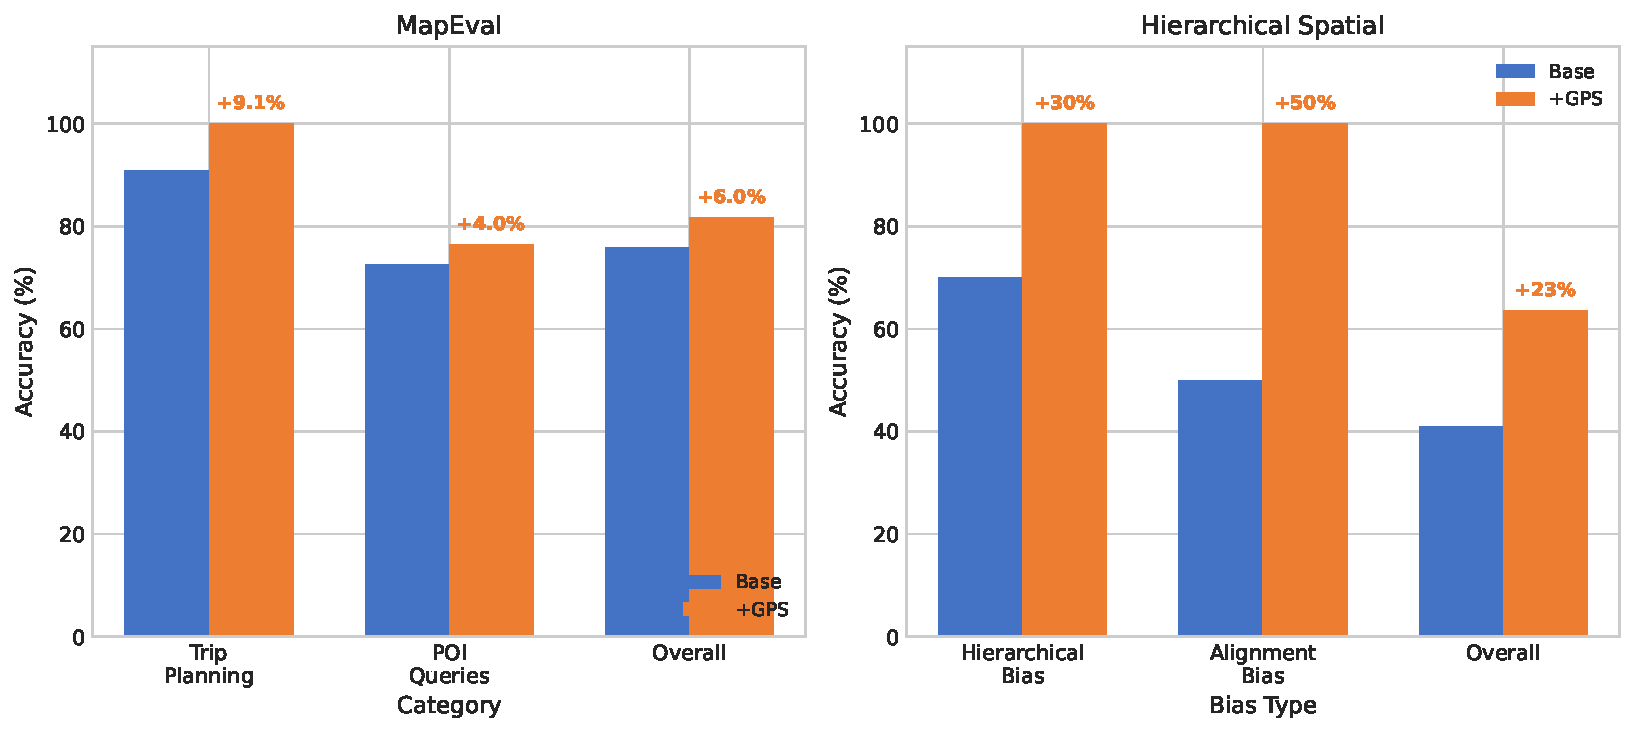
\includegraphics[width=\columnwidth]{figures/downstream_gps_augmentation.pdf}
\caption{Effect of GPS coordinate augmentation on downstream tasks. MapEval shows +6.1\% improvement; Hierarchical Spatial shows +22.7\%, with GPS eliminating hierarchical and alignment biases.}
\label{fig:downstream_gps}
\end{figure}

\paragraph{Findings.}
GPS augmentation produces consistent improvements (Figure~\ref{fig:downstream_gps}). On MapEval, accuracy improves by +6.1\% (75.8\%→81.8\%) when all locations are geocoded. Trip planning benefits most (+9.1\%), as coordinates enable precise distance comparisons. On Hierarchical Spatial, GPS coordinates eliminate hierarchical bias (70\%→100\%) and alignment bias (50\%→100\%). For example, models previously assumed Toronto is north of Portland because Canada is north of the US; with coordinates, they correctly compute that Portland (45.5°N) is north of Toronto (43.7°N). However, proximity and rotation biases remain at 0\%, suggesting these errors stem from deeper spatial reasoning limitations rather than missing coordinate information. Overall, GPS augmentation provides +6--23\% benefit for tasks requiring precise spatial relationships (see Appendix~\ref{app:downstream} for detailed breakdown).

%% =============================================================================
\subsection{RQ4: Can Finetuning Improve GPS Reasoning?}
\label{sec:rq4_finetuning}

We investigate whether task-specific finetuning can improve GPS reasoning by training Qwen3-30B on GPSBench training data and comparing against its zero-shot baseline.

\begin{figure}[htbp]
\centering
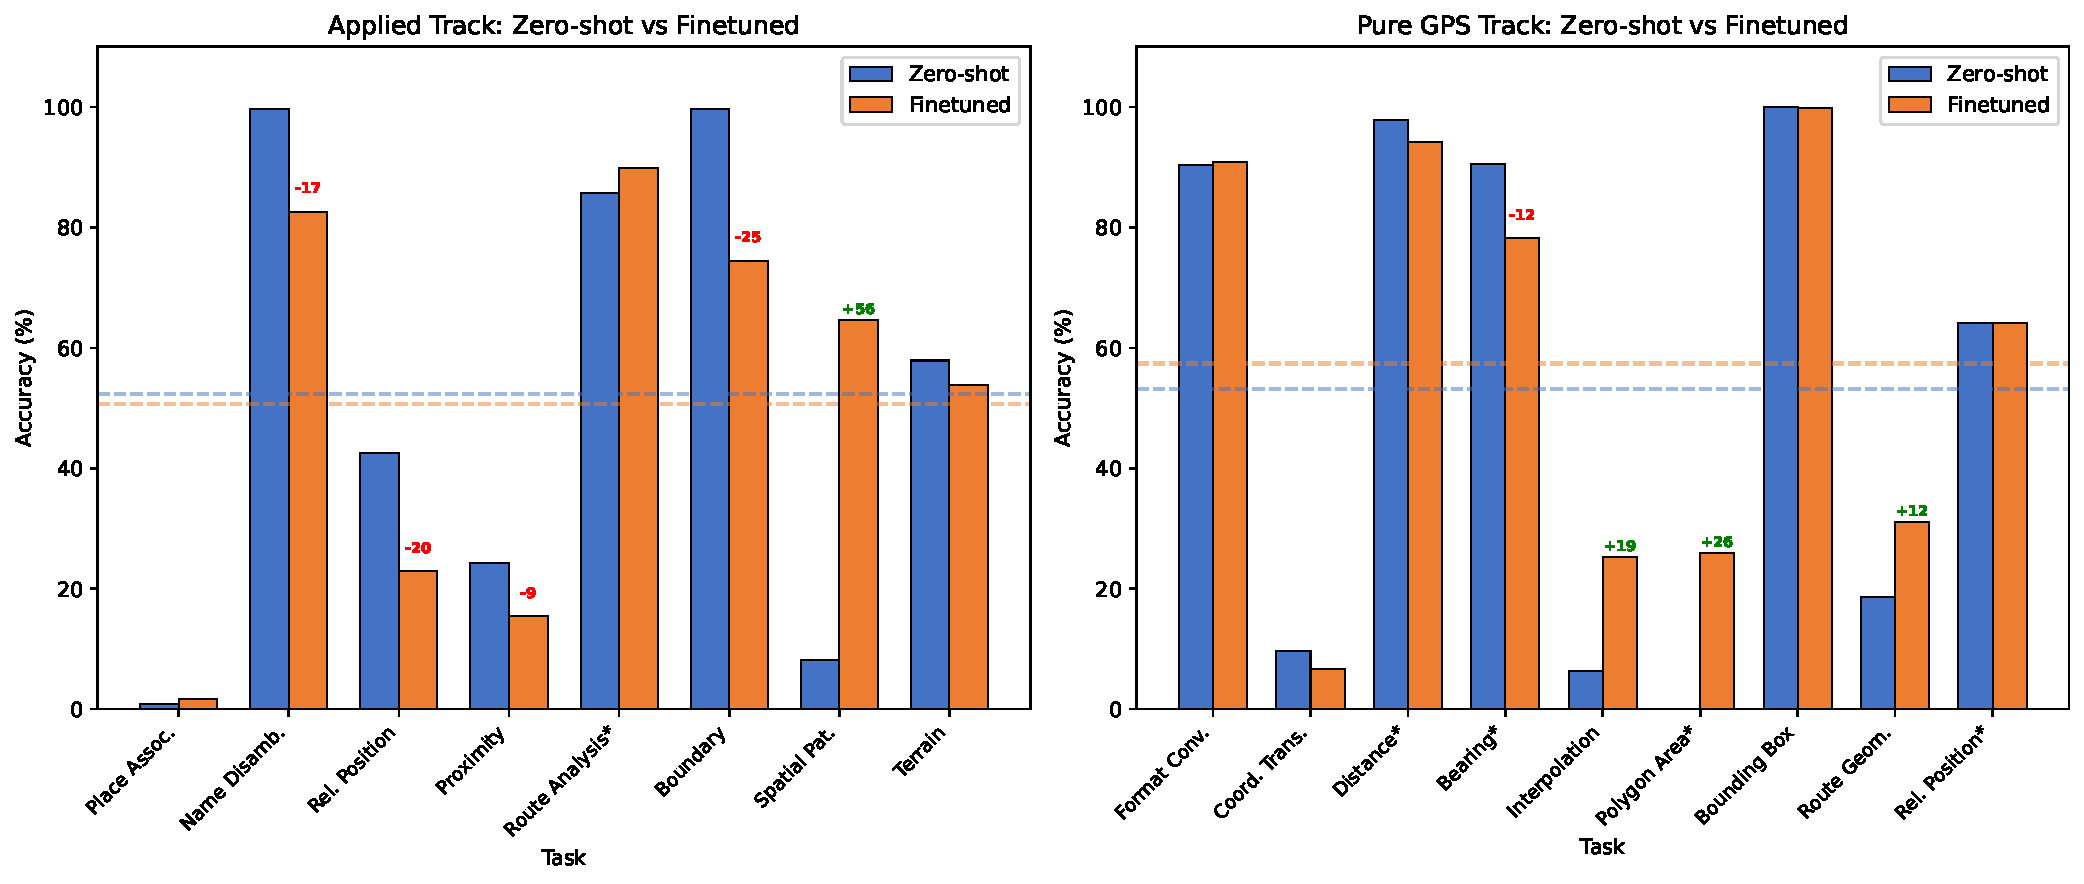
\includegraphics[width=\columnwidth]{figures/finetuning_comparison.pdf}
\caption{Zero-shot vs.\ finetuned Qwen3-30B. Finetuning improves geometric computation (Spatial Patterns +56.5\%, Polygon Area +25.9\%) but degrades world-knowledge tasks (Boundary $-$25.2\%, Name Disambiguation $-$17.1\%).}
\label{fig:finetuning}
\end{figure}

\paragraph{Mixed Results.}
As shown in Figure~\ref{fig:finetuning}, finetuning yields divergent outcomes: Applied Track slightly degrades ($-$1.6\%) while Pure GPS improves (+4.3\%), with +1.5\% net improvement. At the task level, geometric reasoning improves substantially (Spatial Patterns +56.5\%, Polygon Area +25.9\%, Interpolation +18.9\%, Route Geometry +12.4\%), while world-knowledge tasks degrade (Boundary Analysis $-$25.2\%, Relative Position $-$19.6\%, Name Disambiguation $-$17.1\%). Notably, Bearing also degrades ($-$12.3\%) despite being a Pure GPS task, suggesting the improvement pattern is task-specific rather than track-wide.

\paragraph{Capability Trade-offs.}
The pattern suggests finetuning strengthens coordinate computation at the expense of world knowledge integration. Tasks requiring geographic facts (boundaries, place names) suffer catastrophic forgetting, while pure geometric tasks benefit. This highlights that GPS reasoning comprises two distinct capabilities: (1) coordinate manipulation, which is learnable, and (2) geographic knowledge, which risks degradation during finetuning. Future work should explore continual learning techniques to preserve base capabilities while adding GPS skills (see Appendix~\ref{app:finetuning} for per-task breakdown).

%% =============================================================================
\subsection{RQ5: How Does Model Scale Affect GPS Reasoning?}
\label{sec:rq5_scaling}

We analyze scaling behavior using model families with known parameter counts: Mistral (24B, 123B) and Qwen3 (8B, 14B, 30B, 235B).

\begin{figure}[htbp]
\centering
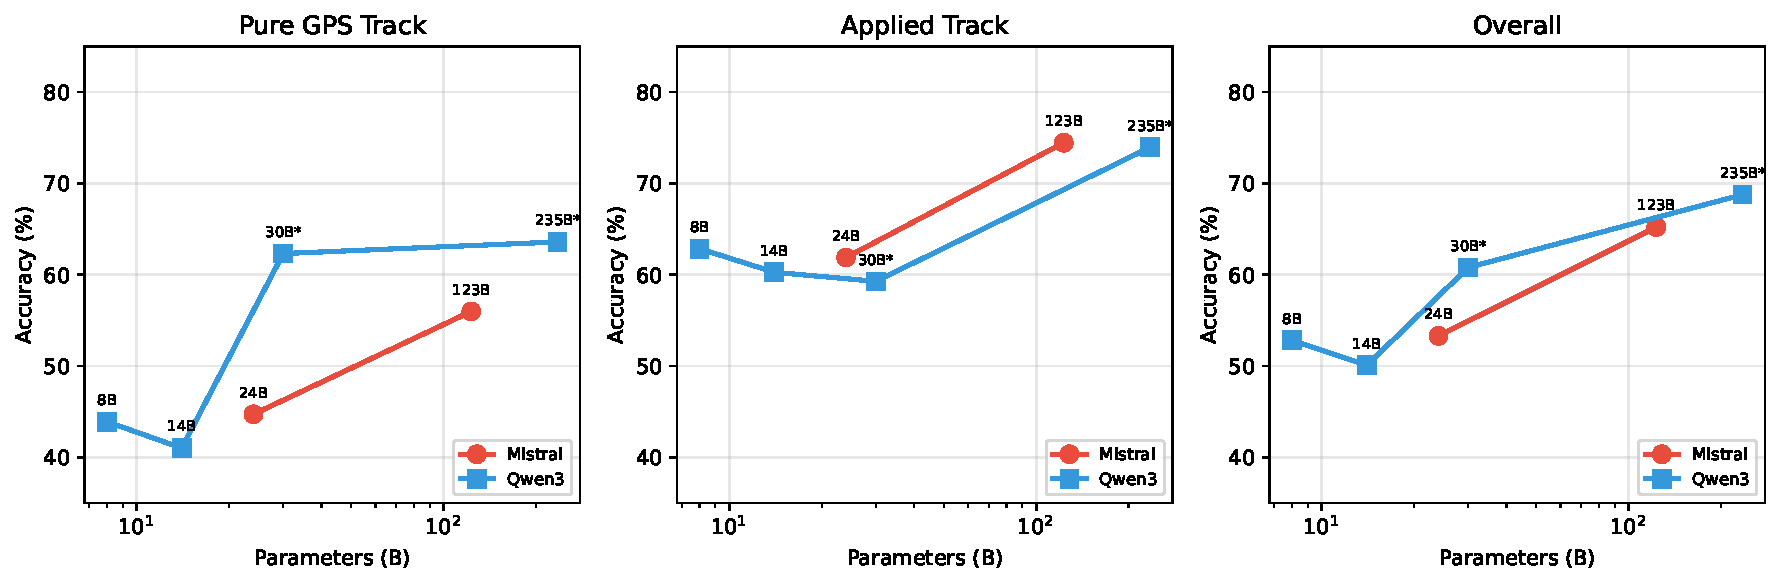
\includegraphics[width=\columnwidth]{figures/scaling_analysis.pdf}
\caption{Scaling analysis for Mistral and Qwen3 model families. Both families show overall improvement with scale, with Qwen3 exhibiting non-monotonic behavior at smaller sizes before improving at larger scales.}
\label{fig:scaling}
\end{figure}

\paragraph{Scaling Patterns.}
As shown in Figure~\ref{fig:scaling}, both model families improve with scale, though with different dynamics. Mistral shows consistent gains with 5.1$\times$ scale-up (24B$\rightarrow$123B): Pure GPS +11.3\%, Applied +12.6\%, Overall +11.9\%. Qwen3 exhibits non-monotonic scaling at smaller sizes (8B$\rightarrow$14B shows slight decrease) but strong improvement at larger scales. Across the full Qwen3 range (8B$\rightarrow$235B, 29$\times$), we observe substantial gains: Pure GPS +19.7\%, Applied +11.1\%, Overall +16.0\%.

\paragraph{Implications.}
The scaling patterns reveal: (1) \textbf{Geographic knowledge scales with parameters}: larger models encode more place-coordinate associations, improving Applied track performance; (2) \textbf{Non-monotonic scaling exists}: smaller model variants may not follow smooth scaling laws, suggesting training dynamics or data mixture effects; (3) \textbf{Both tracks benefit from scale}: unlike some reasoning benchmarks where scaling plateaus, GPS reasoning continues to improve with larger models. These findings suggest that scaling remains an effective strategy for GPS reasoning, though targeted training may be needed for smaller models.
